\pagenumbering{arabic} %設定頁號阿拉伯數字
\setcounter{page}{1}  %設定頁數
\fontsize{12pt}{2.5pt}\sectionef
\section{Process Plan - Production Test Run - Production製程計劃 - 生產試運轉 - 生產}
\fontsize{12}{2.5pt}\selectfont {Now that the prototype phase is complete the focus will shift to the process. As stablished
before, it was decided to separate the prototype products from the final product item to isolate
the product from the production process during the development. This way many aspects of
development of the product could be evaluated in an ordered manner. Now that the process
is been developed it seems reasonable to create the product items that will represent the final
products since the product of a successful run of the process will be the production ready
samples of it (Figure 52). }\\[1pt]

\fontsize{12}{2.5pt}\selectfont {現在原型階段已經完成,將焦點轉移到流程上。如之前所確定的,決定將原型產品與最終產品項目分開,以在開發過程中將產品與生產過程隔離。這樣可以有序地評估產品開發的許多方面。現在流程已經開發,創建代表最終產品的產品項目似乎是合理的,因為成功運行該流程的產品將是其生產就緒樣本(圖52)。}\\[15pt]

\begin{figure}[hbt!]
\begin{center}
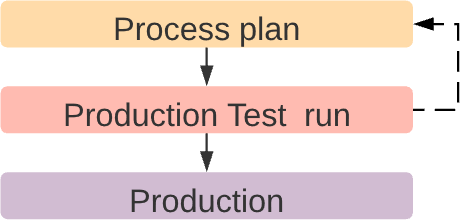
\includegraphics[width=6cm]{52}
\caption{\Large Sectioned diagram regarding Process development 有關流程開發的剖面圖}\label{fig.52}
\end{center}
\end{figure}

\fontsize{12}{2.5pt}\selectfont {Other product items that created were the raw materials for the injection molding (which
are plastic pellets that are fed into the machine to be melted and injected). All that was done
in identical manner to when we create the prototype products with the exception that the
Alpha case (Figure 53) now is marked as sellable and its sale costs are now relevant (Figure
54).  }\\[1pt]

\fontsize{12}{2.5pt}\selectfont {創建的其他產品項目是注塑成型的原材料(其中是送入機器進行熔化和注射的塑膠顆粒)。 一切都已完成與我們創建原型產品時的方式相同,不同之處在於Alpha 案例(圖 53)現在被標記為可銷售,並且其銷售成本現在是相關的(圖54)。}\\[15pt]

\begin{figure}[hbt!]
\begin{center}
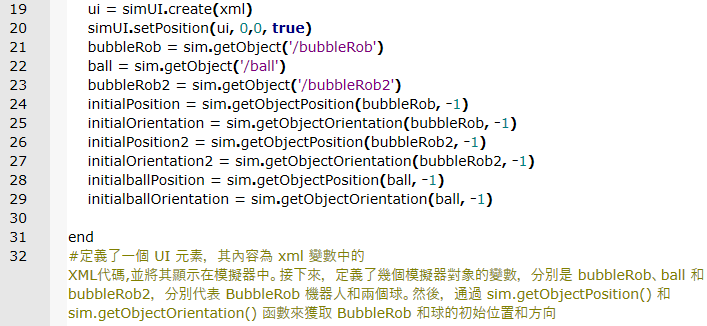
\includegraphics[width=6cm]{53}
\caption{\Large Render of how the final product should look like 最終產品的渲染圖}\label{fig.53}
\end{center}
\end{figure}

\begin{figure}[hbt!]
\begin{center}
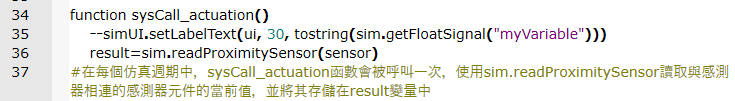
\includegraphics[width=6cm]{54}
\caption{\Large Product Item of the Alpha Case  Alpha Case 的產品項目}\label{fig.54}
\end{center}
\end{figure}

\fontsize{12}{2.5pt}\selectfont {Once the product items are taken care of, we need to go back to what aspect of the process
will be tracked using Odoo in the context of this simulation. As it was hinted previously when
talking about injection molding the key aspect of change regarding the process are the molds
used by the machines to create the parts. For this simulation it was considered that the mold
development will follow a very similar procedure of the development of the product, this
should be more clear from the following diagram (Figure 55). }\\[1pt]

\fontsize{12}{2.5pt}\selectfont {一旦處理完產品項目,我們需要回到流程的哪個方面將在此模擬的上下文中使用 Odoo 進行追蹤。 正如之前所暗示的那樣談論注塑成型過程中變化的關鍵方面是模具被機器用來製造零件。 對於該模擬,認為模具開發將遵循與產品開發非常相似的程序,這從下圖(圖55)應該比較清楚。}\\[15pt]

\begin{figure}[hbt!]
\begin{center}
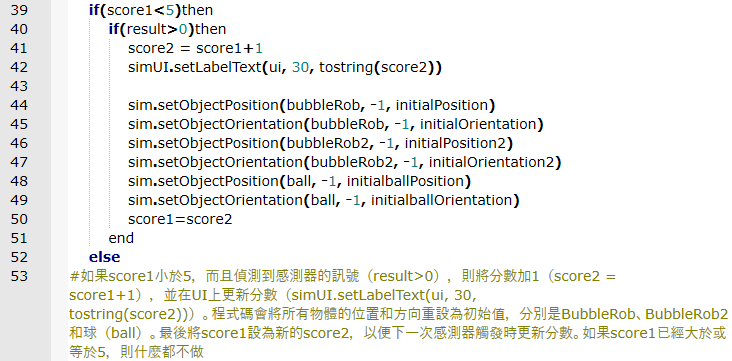
\includegraphics[width=6cm]{55}
\caption{\Large Diagram regarding process development for mold 模具製程開發圖}\label{fig.55}
\end{center}
\end{figure}

\fontsize{12}{2.5pt}\selectfont {The production of a prototype mold by 3D printing follows the same standard procedure
for prototyping used for the product. So far, the mold is considered a product like any other,
this reveals another small weakness regarding Odoo ability to represent the totality of the
process. The reader will notice that although the mold is been treated as a product (because
it is been manufactured) it should in fact be considered a tool or piece of equipment as well. }\\[1pt]

\fontsize{12}{2.5pt}\selectfont {透過 3D 列印生產原型模具遵循相同的標準程序用於產品的原型設計。 到目前為止,模具被認為是與其他產品一樣的產品,這揭示了 Odoo 代表整體能力的另一個小弱點過程。 讀者會注意到,雖然模具被視為產品(因為它已經被製造出來了)事實上它也應該被視為一種工具或設備。}\\[15pt]

\fontsize{12}{2.5pt}\selectfont {Although Odoo does makes this distinction between equipment and products, it has no
integration regarding the situations where one is both. In addition, as explained before, there
is no way of uploading CAD files to an equipment item or linking an equipment to a range
of tools. I.e. Odoo does not consider a vertical drill with x number of drill bits to make
different size holes. The closest it can do from the perspective of equipment/maintenance is
consider the vertical drill a workstation and each drill size a separate equipment within the
station with an assigned set up time. This is ok if you ignore that the drill bit is a product. }\\[1pt]

\fontsize{12}{2.5pt}\selectfont {儘管 Odoo 確實對設備和產品進行了區分,但它沒有關於兩者兼而有之的情況的整合。 另外,如同前面所解釋的,還有無法將 CAD 檔案上傳到裝置項目或將裝置連結到範圍的工具。 IE。 Odoo 不考慮使用 x 鑽頭數量的垂直鑽孔機不同尺寸孔。 從設備/維護的角度來看,它能做的最接近的是將立式鑽孔機視為工作站,並將每個尺寸的鑽孔機視為獨立的設備具有指定設定時間的電台。 如果你忽略了鑽頭是一種產品,這也沒關係。}\\[15pt]

\fontsize{12}{2.5pt}\selectfont {All of this is reasonable from the perspective of an ERP system but not ideal from the
perspective of PLM because it shows gaps in between items that should represent the same
thing. In production from the manufacturing application what is set is the work center station
not the equipment (see Figure 41). In the maintenance app there is no connection to the fact
that the tool is a consumable product, you can consider a maintenance schedule and even
make a useful life parameters but because it is an equipment you can’t have reserve tools
like drill bits in inventory like consumables.}\\[1pt]

\fontsize{12}{2.5pt}\selectfont {這一切從ERP系統的角度來看是合理的,但從實際應用角度來看卻不理想。PLM 的視角,因為它顯示了應該代表相同內容的項目之間的差距事物。 在製造應用程式的生產中,設置的是工作中心站不是設備(參見圖 41)。 在維護應用程式中,與事實無關該工具是消耗品,您可以考慮維護計劃,甚至制定使用壽命參數,但因為它是設備,所以不能有備用工具就像庫存中的鑽頭一樣,就像消耗品一樣。}\\[15pt]

\fontsize{12}{2.5pt}\selectfont {The result is that it becomes very difficult to represent testing with a prototype mold. If
you do as the software is designed for you need to create a separate ECO to apply every
operation for each different iteration of the mold development to the necessary BOMs and
make a test run (Figure 56). At this point, considering the maintenance aspect of the mold as
a tool just does not make sense because it would entails filing in metadata in the maintenance
App by hand for every prototype mold iteration all without causing any difference from the
manufacturing perspective. The PROTO mold item ends up been used only for the sake of
tracking material and holding files as the mold is improved. }\\[1pt]

\fontsize{12}{2.5pt}\selectfont {結果是用原型模具來表示測試變得非常困難。 如果您所做的,因為該軟體是為您需要建立一個單獨的 ECO 來應用每個模具開發的每個不同迭代的操作都需要必要的 BOM 和進行測試運行(圖 56)。 此時,考慮到模具的維護面工具沒有意義,因為它需要在維護中歸檔元數據為每個原型模具迭代手動應用程序,不會造成與實際模型的任何差異製造角度。 原型模具專案最終僅用於隨著模具的改進,追蹤材料並保存文件。}\\[15pt]
\newpage
\begin{figure}[hbt!]
\begin{center}
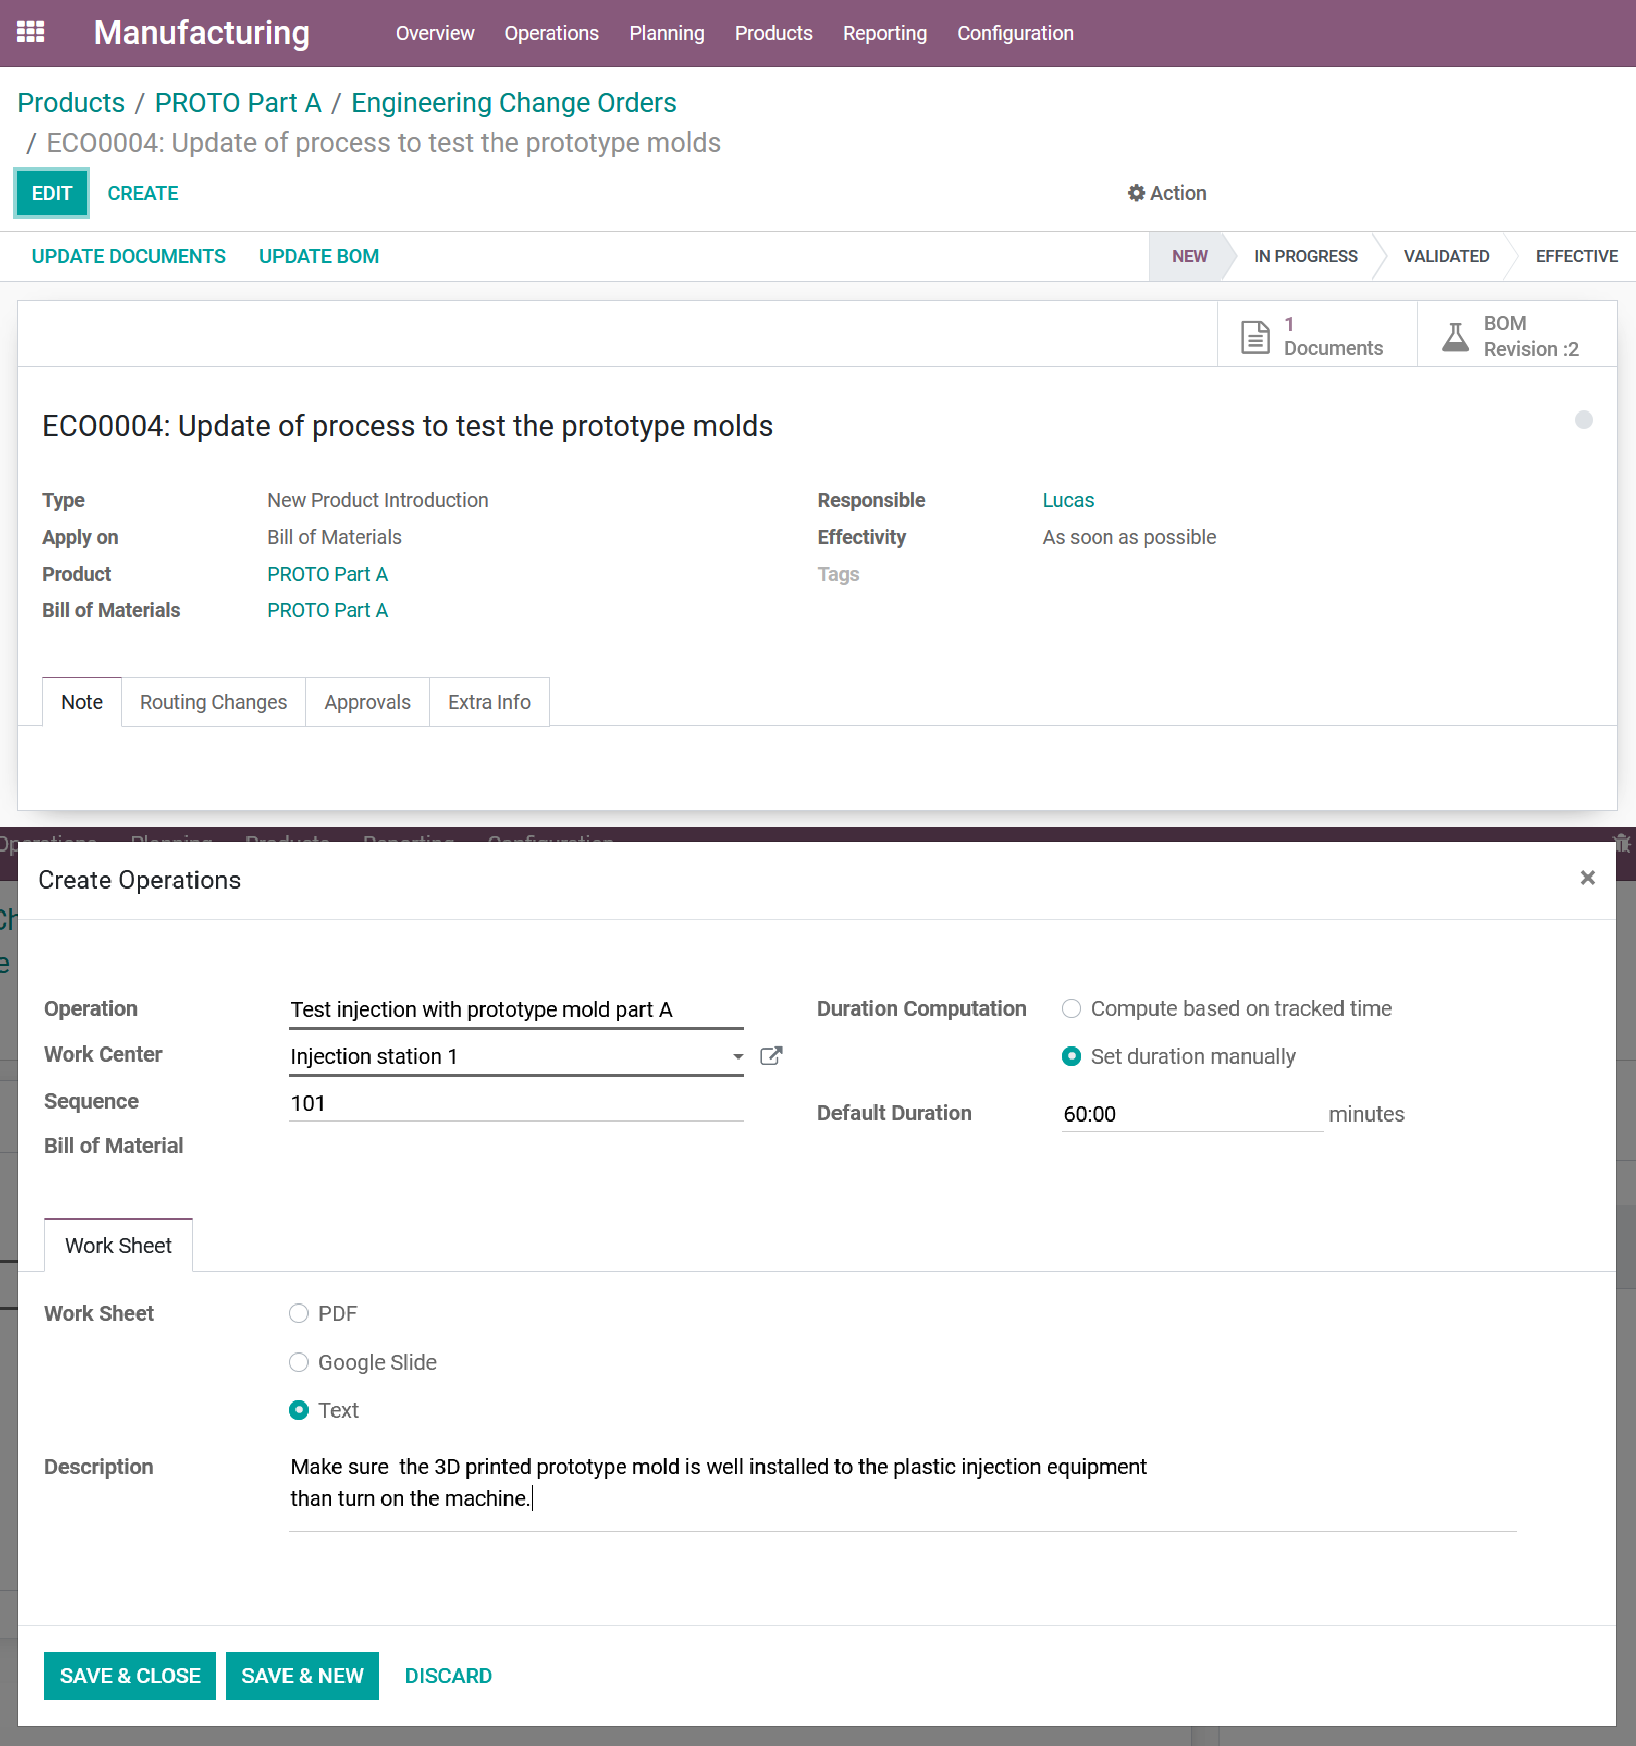
\includegraphics[width=6cm]{56}
\caption{\Large ECO example of update procedure of BOM BOM更新流程ECO範例}\label{fig.56}
\end{center}
\end{figure}

\fontsize{12}{2.5pt}\selectfont {Taking this in consideration, in simulation it will be produced one 3D printed mold for
each part of the alpha case. Then ECOs for the prototype parts of the case will be created to
be applied to the parts BOMs updating the operation from 3D printing to injection molding
test run with prototype molds.}\\[1pt]

\fontsize{12}{2.5pt}\selectfont {考慮到這一點,在模擬中將生產一個 3D 列印模具alpha 案例的每個部分。 然後將創建案例原型部分的 ECO適用於零件 BOM,將操作從 3D 列印更新為射出成型使用原型模具進行試運行。}\\[15pt]

\fontsize{12}{2.5pt}\selectfont {At this point we could differentiate the product prototype from the test run prototype by
making a new prototype product item, however considering our rapidly growing list of
product items (Figure 57) it was concluded that it would be just better for depiction in this
work to modify the previously produced product prototypes (made with 3D printing) and justuse the same items. We can do this because those prototypes have already served their
purpose.  }\\[1pt]

\fontsize{12}{2.5pt}\selectfont {此時,我們可以透過以下方式區分產品原型和試運行原型:製作一個新的原型產品項目,但考慮到我們快速成長的列表產品項目(圖 57)的結論是,在此描述會更好修改先前製作的產品原型(透過 3D 列印製作)並僅使用相同的物品。 我們可以做到這一點,因為這些原型已經投入使用目的。}\\[15pt]
\newpage
\begin{figure}[hbt!]
\begin{center}
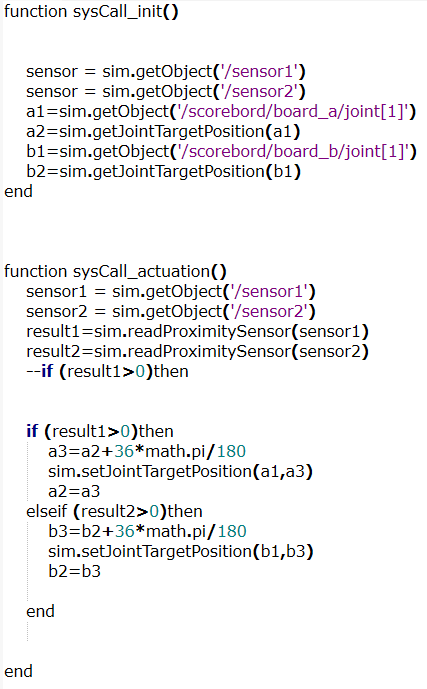
\includegraphics[width=6cm]{57}
\caption{\Large Overview of product items at this stage of the simulation 模擬此階段的產品項目概述}\label{fig.57}
\end{center}
\end{figure}

\fontsize{12}{2.5pt}\selectfont {After the mold have been created and the BOMs for the prototypes are updated to include
the injection stations and the proper operations (specifying the use of the molds) the next step
is to do a production test run of prototype. Again that is done by emitting the MO completing
the generated WOs (see Figure 46 and Figure 47 of previous section). }\\[1pt]

\fontsize{12}{2.5pt}\selectfont {創建模具並更新原型的 BOM 後,包括注射站和正確的操作(指定模具的使用)下一步是對原型進行生產測試。 同樣,這是透過發出 MO 完成來完成的生成的 WO(參見上一節的圖 46 和圖 47)。}\\[15pt]

\fontsize{12}{2.5pt}\selectfont {The result of the production is used to check for dimension and fitting, if correction is
needed the ECOs would be emitted again as seen in Figure 56, and a new iteration of
production and testing would be carried out. This process would repeat until the product is
satisfactory enough to justify the production of the CNC machined molds that would be used
in mass production.  }\\[1pt]

\fontsize{12}{2.5pt}\selectfont {生產結果用於檢查尺寸和配合,如果修正的話需要再次發出 ECO,如圖 56 所示,並且新的迭代將進行生產和測試。 這個過程會重複,直到產品被足以證明所使用的 CNC 加工模具的生產是合理的在批量生產中。}\\[15pt]

\fontsize{12}{2.5pt}\selectfont {Since in this simulation it was chosen that the final mold (made of aluminum) would also
be produced in house, this is the next step of development. Procedure is basically the same
as before except that it is needed to create product items for both the raw material (aluminum
block) and the CNC molds prior to their manufacturing. Creating BOMs and uploading
relevant files. }\\[1pt]

\fontsize{12}{2.5pt}\selectfont {由於在此模擬中選擇最終模具(由鋁製成)也將內部生產,這是下一步的開發。 流程基本相同與以前一樣,只是需要為原材料(鋁)創建產品項目塊)和製造前的 CNC 模具。 建立 BOM 並上傳相關文件。}\\[15pt]

\fontsize{12}{2.5pt}\selectfont {Finally, the actual production on the new molds can begin. To represent that a
manufacturing order of 100 Alpha Cases were created. This marks the end of the main path
of development from idea to production (Figure 58).}\\[1pt]

\fontsize{12}{2.5pt}\selectfont {最後,新模具可以開始實際生產。 來表示一個創建了 100 個 Alpha Case 的製造訂單。 這標誌著主路徑的結束從創意到生產的開發過程(圖 58)。}\\[15pt]

\begin{figure}[hbt!]
\begin{center}
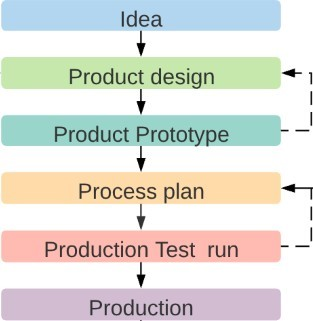
\includegraphics[width=6cm]{58}
\caption{\Large Main path of development from idea to production 從創意到生產的主要發展路徑}\label{fig.58}
\end{center}
\end{figure}
